\let\lesson\undefined
\newcommand{\lesson}{\phantomlesson{Bài 4: Chuyển động thẳng}}
\chapter[Độ dịch chuyển và quãng đường]{Độ dịch chuyển và quãng đường đi được}
\setcounter{section}{0}
\section{Lý thuyết}
\subsection{Chuyển động cơ. Chất điểm}
\subsubsection{Chuyển động cơ}
Chuyển động cơ của một vật (gọi tắt là chuyển động) là sự thay đổi vị trí của vật đó so với các vật khác theo thời gian.
\subsubsection{Chất điểm}
Một vật chuyển động được coi là một chất điểm nếu kích thước của nó rất nhỏ so với độ dài đường đi (hoặc so với những khoảng cách mà ta đề cập đến).

Ví dụ: trong chuyển động của ô tô từ thành phố Hồ Chí Minh đến Hà Nội thì ô tô được xem là chất điểm.
\subsubsection{Quỹ đạo}
Tập hợp tất cả các vị trí của một chất điểm chuyển động tạo ra một đường trong không gian, đường đó gọi là quỹ đạo của chuyển động.
\subsection{Cách xác định vị trí của vật trong không gian}
\subsubsection{Vật làm mốc và thước đo}
Nếu đã biết đường đi (quỹ đạo) của vật, ta cần chọn một vật làm mốc và một chiều dương trên đường đi, và dùng thước đo chiều dài đoạn đường từ vật làm mốc đến vật là có thể xác định được chính xác vị trí của vật.
\begin{center}
	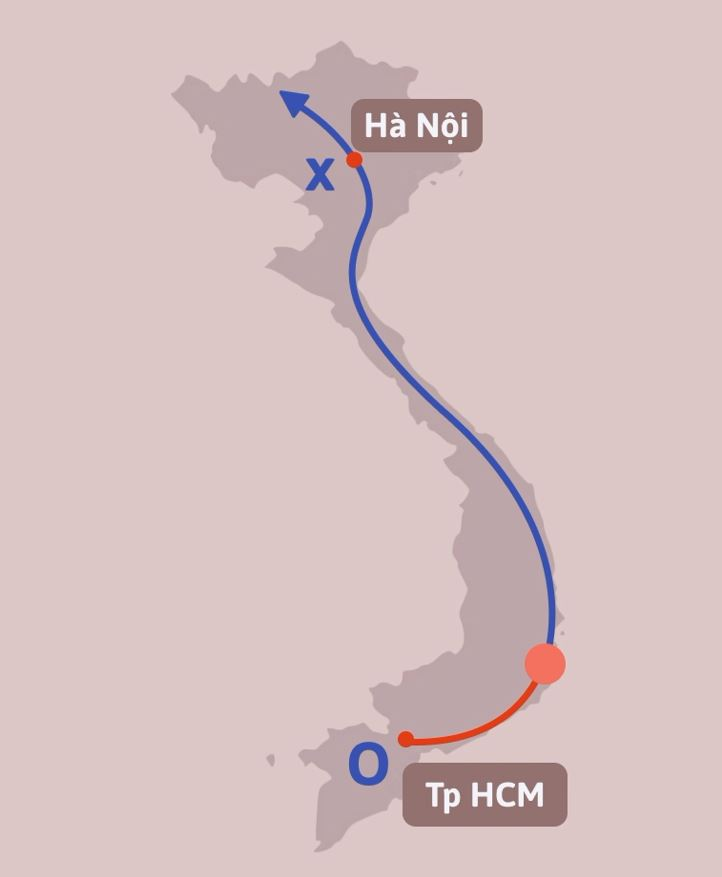
\includegraphics[scale=0.3]{../figs/VN10-PH-02-L-001-1-V2-01.jpg}
\end{center}
\subsubsection{Hệ tọa độ}
Muốn xác định vị trí của một điểm trên một mặt phẳng ta cần có hệ tọa độ với hai trục O$x$ và O$y$ vuông góc nhau, hình chiếu vuông góc của điểm xuống hai trục tọa độ đó chính là tọa độ của điểm đó.
\begin{center}
	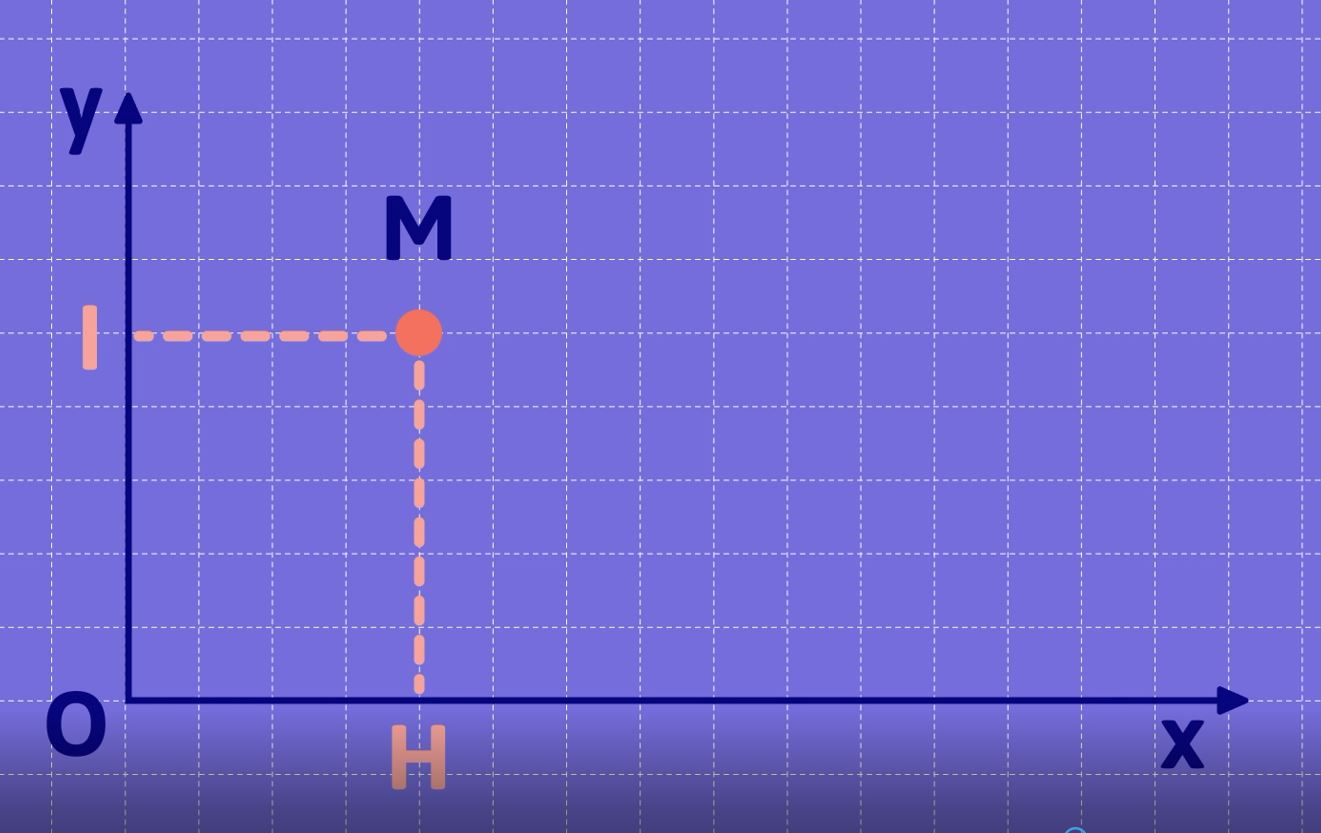
\includegraphics[height=3cm]{../figs/VN10-PH-02-L-001-1-V2-02.jpg}
	
\end{center}
\subsection{Cách xác định thời gian trong chuyển động}
\subsubsection{Mốc thời gian và đồng hồ}
Để mô tả chuyển động của một vật ta phải biết tọa độ của vật đó ở những thời điểm khác nhau. Muốn thế, ta phải chỉ rõ mốc thời gian và đo khoảng thời gian trôi đi kể từ mốc thời gian bằng một đồng hồ.
\subsubsection{Thời điểm và thời gian}
Nếu lấy mốc thời gian là thời điểm vật bắt đầu chuyển động (thời điểm 0) thì số chỉ của thời điểm sẽ trùng với số đo khoảng thời gian đã trôi qua kể từ mốc thời gian.
\subsection{Hệ quy chiếu}
Một hệ quy chiếu gồm:
\begin{itemize}
	\item mốc tọa độ và một hệ tọa độ để đo vị trí;
	\item mốc thời gian và một đồng hồ để xác định thời điểm.
\end{itemize}
\subsection{Độ dịch chuyển và quãng đường đi được}
\subsubsection{Độ dịch chuyển}
Độ dịch chuyển được xác định bằng độ biến thiên toạ độ của vật
$$d=x_2-x_1=\Delta x$$
\begin{center}
	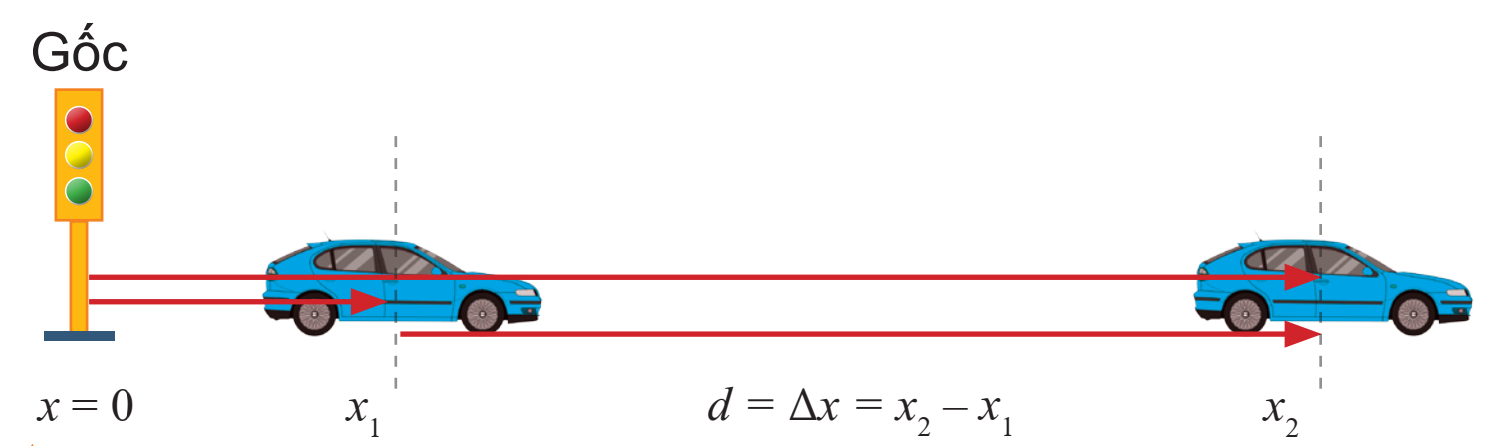
\includegraphics[width=0.6\linewidth]{../figs/VN10-2023-PH-TP004-1}
	\captionof{figure}{Ví dụ thực tế về độ dịch chuyển của vật trên đường thẳng}
\end{center}
Độ dịch chuyển có các đặc điểm sau:
\begin{itemize}
	\item độ dịch chuyển là một đại lượng vectơ $\left(\vec{d}\right)$ có gốc tại vị trí ban đầu, hướng từ vị trí đầu đến vị trí cuối, độ lớn bằng khoảng cách giữa vị trí đầu và vị trí cuối.
	\item độ dịch chuyển là một đại lượng có thể nhận giá trị dương, âm hoặc bằng không. 
\end{itemize}
\subsubsection{So sánh độ dịch chuyển và quãng đường đi được}
\begin{longtable}{|m{20em}|m{20em}|}
	\hline
	\thead{Độ dịch chuyển $\left(\vec{d}\right)$} & \thead{Quãng đường $\left(s\right)$}\\
	\hline
	Là đại lượng vectơ. & Là đại lượng vô hướng.\\
	\hline
	Cho biết sự thay đổi vị trí của một vật (về hướng và độ dời). & Cho biết độ dài mà vật đi được.\\
	\hline
	Có thể nhận giá trị dương, âm hoặc bằng 0. & Có giá trị không âm.\\
	\hline
\end{longtable}
\luuy{Khi vật chuyển động theo một hướng (chuyển động thẳng và không đổi chiều) thì độ lớn của độ dịch chuyển và quãng đường đi được bằng nhau $(d=s)$.

}
\section{Mục tiêu bài học - Ví dụ minh họa}
\begin{dang}{Thực hiện xác định thời điểm và thời gian (mốc thời gian và đồng hồ)}
	\viduii{2}{Giờ Berlin chậm hơn giờ Hà Nội 5 giờ. Trận bóng đá diễn ra tại Beclin lúc 19h00 ngày 2-9-2021. Khi đó theo giờ Hà Nội là
		\begin{mcq}(2)
			\item 14h00 ngày 3-9-2021.
			\item 0h00 ngày 3-9-2021. 
			\item 0h00 ngày 2-9-2021
			\item 14h00 ngày 2-9-2021.
		\end{mcq}
	}
	{\hide{	
		Giờ Berlin chậm hơn giờ Hà Nội 5 giờ, nghĩa là
		$$t_{\text{B}}+\SI{5}{\hour}=t_{\text{HN}}.$$
		Trận bóng đá diễn ra tại Berlin lúc 19h00 ngày 2-9-2021. Thời điểm đó theo giờ Hà Nội là:
		$$t_{\text{HN}}=t_{\text{B}}+\SI{5}{\hour}=19\text{h}00 + 5\text{h} = 24\text{h}00$$
		Một ngày chỉ có 24 giờ nên thời điểm trên đã bước sang ngày hôm sau. Do đó, trận bóng trên diễn ra vào lúc 0h00 ngày 3-9-2007 giờ Hà Nội. 	
		
		\textbf{Đáp án: B}.
	}}

	\viduii{3}{Theo lịch trình tại bến xe ở Hà Nội thì ô tô chở khách trên tuyến Hà Nội - Hải Phòng chạy từ Hà Nội lúc 6 giờ sáng, đi qua Hải Dương lúc 7 giờ 15 phút sáng và tới Hải Phòng lúc 8 giờ 50 phút sáng cùng ngày. Hà Nội cách Hải Dương 60 km và cách Hải Phòng $\SI{105}{km}$. Xe ô tô chạy liên tục không nghỉ dọc đường, chỉ dừng lại 10 phút tại bến xe Hải Dương để đón, trả khách. Tính khoảng thời gian chuyển động và quãng đường đi được của các hành khách sau:
		\begin{enumerate}[label=\alph*)]
			\item Hành khách lên xe tại Hà Nội đi Hải Phòng.
			\item Hành khách lên xe tại Hải Dương đi Hải Phòng.
		\end{enumerate}
	}
	{\hide{
		\begin{enumerate}[label=\alph*)]
			\item Đối với hành khách lên xe tại Hà Nội đi Hải Phòng, chọn bến xe Hà Nội làm mốc và thời điểm ô tô bắt đầu xuất phát là mốc thời gian.
			
			Khoảng thời gian chuyển động là:	
			\begin{center}
				(8 giờ 50 phút - 6 giờ) - 10 phút = 2 giờ 40 phút.
			\end{center}
			Quãng đường đi được đúng bằng độ dài của đoạn đường Hà Nội - Hải Phòng là $\SI{105}{km}$.
			\item Đối với hành khách lên xe tại Hải Dương đi Hải Phòng, chọn bến xe Hải Dương làm mốc và thời điểm ô tô bắt đầu xuất phát là mốc thời gian.
			
			Khoảng thời gian chuyển động là:
			\begin{center}
				8 giờ 50 phút - (7 giờ 15 phút + 10 phút) = 1 giờ 25 phút.
			\end{center}
			Quãng đường đi được là:
			$$\SI{105}{km}-\SI{60}{km}=\SI{45}{km}.$$
		\end{enumerate}
	}}
\end{dang}

\begin{dang}{So sánh được quãng đường đi được và độ dịch chuyển.}
	\viduii{2}
{Xét quãng đường $AB$ dài $\SI{1000}{\meter}$ với $A$ là vị trí nhà của em và $B$ là vị trí của bưu điện. Tiệm tạp hóa nằm tại vị trí $C$ là trung điểm của $AB$. Nếu chọn nhà em làm gốc tọa độ và chiều dương hướng từ nhà em đến bưu điện. Hãy xác định độ dịch chuyển và quãng đường đi được của em trong các trường hợp:
	\begin{center}
		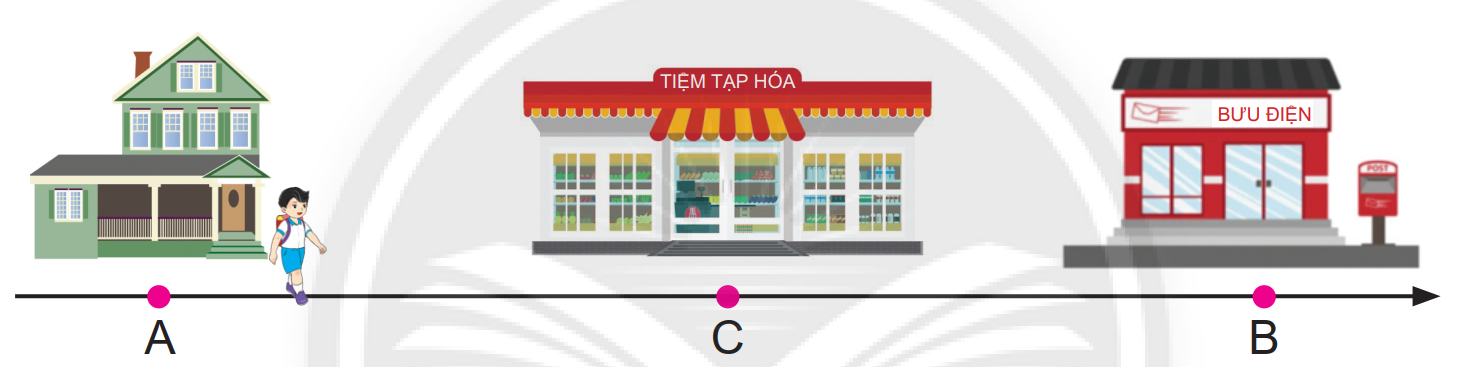
\includegraphics[width=0.6\linewidth]{../figs/VN10-2023-PH-TP004-2}
	\end{center}
	\begin{enumerate}[label=\alph*)]
		\item Đi từ nhà đến bưu điện.
		\item Đi từ nhà đến bưu điện rồi quay lại tiệm tạp hóa.
		\item Đi từ nhà đến tiệm tạp hóa rồi quay về. 
	\end{enumerate}	
}
{\hide{
\begin{enumerate}[label=\alph*)]
	\item Độ dịch chuyển $d=AB=x_B-x_A=\SI{1000}{\meter}-\SI{0}{\meter}=\SI{1000}{\meter}$.\\
	Quãng đường đi được $s=AB=\SI{1000}{\meter}$.
	\item Độ dịch chuyển $d=AC=x_A-x_C=\SI{500}{\meter}-\SI{0}{\meter}=\SI{500}{\meter}$.\\
	Quãng đường đi được $s=AB+BC=\SI{1500}{\meter}$.
	\item  Độ dịch chuyển $d=x_A-x_A=\SI{0}{\meter}$.\\
	Quãng đường đi được $s=2AC=\SI{1000}{\meter}$.
\end{enumerate}
}}

\viduii{2}
{Một vận động viên chạy từ cổng Dinh Thống Nhất (A) đến Thảo Cầm Viên (D) theo hai quỹ đạo khác nhau. Hãy xác định độ dịch chuyển và quãng đường chạy được của người vận động viên trong 2 trường hợp trên.
\begin{center}
	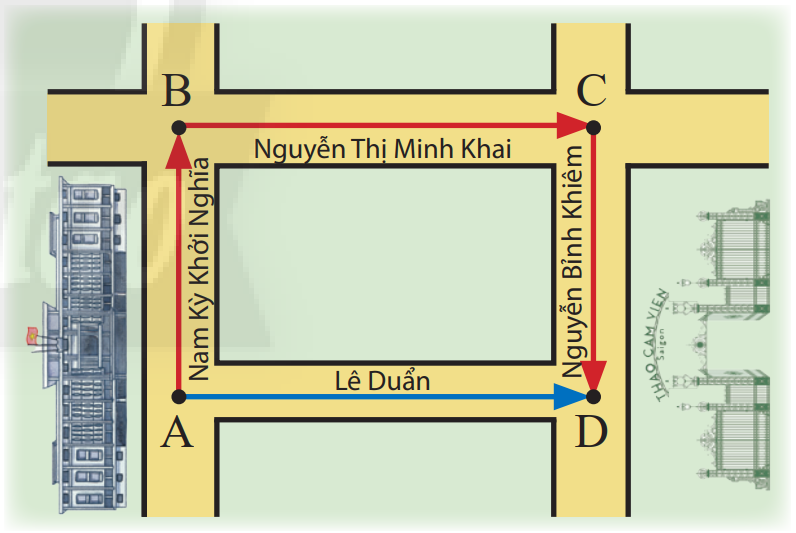
\includegraphics[width=0.5\linewidth]{../figs/VN10-2023-PH-TP004-3}
\end{center}
}
{\hide{
\textbf{Trường hợp 1:} Nếu vận động viên chạy theo đường Lê Duẩn thì\\
	Độ dời $\vec{d}=\overrightarrow{AD}$, về độ lớn thì $d=AD$.\\
	Quãng đường $s=AD$.\\
\textbf{Trường hợp 2:} Nếu vận động viên chạy theo đường Nam Kì Khởi Nghĩa qua đường Nguyễn Thị Minh Khai rồi mới đến Thảo Cầm Viên ở đường Nguyễn Bỉnh Khiêm thì\\
Độ dời $\vec{d}=\overrightarrow{AD}$, về độ lớn thì $d=AD$.\\
Quãng đường $s=AB+BC+CD$.
}}
\end{dang}

